% !TEX TS-program = XeLaTeX
% use the following command: 
% all document files must be coded in UTF-8
\documentclass{textolivre}
% for anonymous submission
%\documentclass[anonymous]{textolivre}
% to create HTML use 
%\documentclass{textolivre-html}
% See more information on the repository: https://github.com/leolca/textolivre

% Metadata
\begin{filecontents*}[overwrite]{article.xmpdata}
    \Title{A convergência tecnológica e digital, o ensino remoto emergencial e os alunos com TDAH que frequentam os anos finais do ensino fundamental}
    \Author{Sineide Gonçalves \sep Bárbara Eduarda Barbosa Ferreira}
    \Language{pt-BR}
    \Keywords{TDAH \sep Educação inclusiva \sep Convergência digital \sep COVID-19}
    \Journaltitle{Texto Livre}
    \Journalnumber{1983-3652}
    \Volume{14}
    \Issue{1}
    \Firstpage{1}
    \Lastpage{16}
    \Doi{10.35699/1983-3652.2021.25043}

    \setRGBcolorprofile{sRGB_IEC61966-2-1_black_scaled.icc}
            {sRGB_IEC61966-2-1_black_scaled}
            {sRGB IEC61966 v2.1 with black scaling}
            {http://www.color.org}
\end{filecontents*}

% used to create dummy text for the template file
\definecolor{dark-gray}{gray}{0.35} % color used to display dummy texts
\usepackage{lipsum}
\SetLipsumParListSurrounders{\colorlet{oldcolor}{.}\color{dark-gray}}{\color{oldcolor}}

% used here only to provide the XeLaTeX and BibTeX logos
\usepackage{hologo}

% used in this example to provide source code environment
%\crefname{lstlisting}{lista}{listas}
%\Crefname{lstlisting}{Lista}{Listas}
%\usepackage{listings}
%\renewcommand\lstlistingname{Lista}
%\lstset{language=bash,
        breaklines=true,
        basicstyle=\linespread{1}\small\ttfamily,
        numbers=none,xleftmargin=0.5cm,
        frame=none,
        framexleftmargin=0.5em,
        framexrightmargin=0.5em,
        showstringspaces=false,
        upquote=true,
        commentstyle=\color{gray},
        literate=%
           {á}{{\'a}}1 {é}{{\'e}}1 {í}{{\'i}}1 {ó}{{\'o}}1 {ú}{{\'u}}1 
           {à}{{\`a}}1 {è}{{\`e}}1 {ì}{{\`i}}1 {ò}{{\`o}}1 {ù}{{\`u}}1
           {ã}{{\~a}}1 {ẽ}{{\~e}}1 {ĩ}{{\~i}}1 {õ}{{\~o}}1 {ũ}{{\~u}}1
           {â}{{\^a}}1 {ê}{{\^e}}1 {î}{{\^i}}1 {ô}{{\^o}}1 {û}{{\^u}}1
           {ä}{{\"a}}1 {ë}{{\"e}}1 {ï}{{\"i}}1 {ö}{{\"o}}1 {ü}{{\"u}}1
           {Á}{{\'A}}1 {É}{{\'E}}1 {Í}{{\'I}}1 {Ó}{{\'O}}1 {Ú}{{\'U}}1
           {À}{{\`A}}1 {È}{{\`E}}1 {Ì}{{\`I}}1 {Ò}{{\`O}}1 {Ù}{{\`U}}1
           {Ã}{{\~A}}1 {Ẽ}{{\~E}}1 {Ũ}{{\~u}}1 {Õ}{{\~O}}1 {Ũ}{{\~U}}1
           {Â}{{\^A}}1 {Ê}{{\^E}}1 {Î}{{\^I}}1 {Ô}{{\^O}}1 {Û}{{\^U}}1
           {Ä}{{\"A}}1 {Ë}{{\"E}}1 {Ï}{{\"I}}1 {Ö}{{\"O}}1 {Ü}{{\"U}}1
           {ç}{{\c{c}}}1 {Ç}{{\c{C}}}1
}


\journalname{Texto Livre: Linguagem e Tecnologia}
\thevolume{14}
\thenumber{1}
\theyear{2021}
\receiveddate{\DTMdisplaydate{2020}{8}{30}{-1}} % YYYY MM DD
\accepteddate{\DTMdisplaydate{2021}{1}{28}{-1}}
\publisheddate{\today}
% Corresponding author
\corrauthor{Sineide Gonçalves}
% DOI
\articledoi{10.35699/1983-3652.2021.25043}
% list of available sesscions in the journal: articles, dossier, reports, essays, reviews, interviews, editorial
\articlesessionname{Educação e Tecnologia}
% Abbreviated author list for the running footer
\runningauthor{Gonçalves e Ferreira}
\editorname{Daniervelin Pereira}

\title{A convergência tecnológica e digital, o ensino remoto emergencial e os alunos com TDAH que frequentam os anos finais do ensino fundamental}
\othertitle{Technological and digital convergence, emergency remote education and ADHD students who attend the final years of elementary school}
% if there is a third language title, add here:
%\othertitle{Artikelvorlage zur Einreichung beim Texto Livre Journal}

\author[1]{Sineide Gonçalves \orcid{0000-0002-4067-5358} \thanks{Email: \url{sineide.ufmg@gmail.com}}}
\author[2]{Bárbara Eduarda Barbosa Ferreira \orcid{0000-0003-1569-9638} \thanks{Email: \url{pedagogabarbaraa@gmail.com}}}

\affil[1]{Universidade Federal de Minas Gerais, Belo Horizonte, MG, Brasil.}
\affil[2]{Universidade Federal de Ouro Preto, Ouro Preto, MG, Brasil.}

\addbibresource{article.bib}
% use biber instead of bibtex
% $ biber tl-article-template

% set language of the article
\setdefaultlanguage[variant=brazilian]{portuguese}
\setotherlanguage{english}

% for spanish, use:
%\setdefaultlanguage{spanish}
%\gappto\captionsspanish{\renewcommand{\tablename}{Tabla}} % use 'Tabla' instead of 'Cuadro'

% for languages that use special fonts, you must provide the typeface that will be used
% \setotherlanguage{arabic}
% \newfontfamily\arabicfont[Script=Arabic]{Amiri}
% \newfontfamily\arabicfontsf[Script=Arabic]{Amiri}
% \newfontfamily\arabicfonttt[Script=Arabic]{Amiri}
%
% in the article, to add arabic text use: \textlang{arabic}{ ... }

% to use emoticons in your manuscript
% https://stackoverflow.com/questions/190145/how-to-insert-emoticons-in-latex/57076064
% using font Symbola, which has full support
% the font may be downloaded at:
% https://dn-works.com/ufas/
% add to preamble:
% \newfontfamily\Symbola{Symbola}
% in the text use:

% reference itens in a descriptive list using their labels instead of numbers
% insert the code below in the preambule:
%
\makeatletter
\let\orgdescriptionlabel\descriptionlabel
\renewcommand*{\descriptionlabel}[1]{%
  \let\orglabel\label
  \let\label\@gobble
  \phantomsection
  \edef\@currentlabel{#1\unskip}%
  \let\label\orglabel
  \orgdescriptionlabel{#1}%
}
\makeatother
%
% in your document, use as illustraded here:
%\begin{description}
%  \item[first\label{itm1}] this is only an example;
%  % ...  add more items
%\end{description}

% custom epigraph - BEGIN 
%%% https://tex.stackexchange.com/questions/193178/specific-epigraph-style
\usepackage{epigraph}
\renewcommand\textflush{flushright}
\makeatletter
\newlength\epitextskip
\pretocmd{\@epitext}{\em}{}{}
\apptocmd{\@epitext}{\em}{}{}
\patchcmd{\epigraph}{\@epitext{#1}\\}{\@epitext{#1}\\[\epitextskip]}{}{}
\makeatother

\setlength\epigraphrule{0pt}
\setlength\epitextskip{0.5ex}
\setlength\epigraphwidth{.7\textwidth}
% custom epigraph - END

\begin{document}
\maketitle

\begin{polyabstract}
\begin{abstract}
Este artigo contempla algumas práticas educacionais inclusivas que permeiam a cibercultura voltadas para alunos com NEE (Necessidades Educacionais Especiais), dando ênfase aos alunos com TDAH (Transtorno do Déficit de Atenção com Hiperatividade) que frequentam os anos finais do Ensino Fundamental. O objetivo é mostrar alguns recursos digitais que podem incentivar estes alunos a ler e escrever a partir da educação remota. Ao abordar algumas especificidades e contribuições do letramento digital no processo de ensino/aprendizagem e sua relação com um mundo que está passando, simultaneamente, por uma pandemia causada pela COVI-19 e por uma progressiva convergência tecnológica, concluímos que a maioria das ferramentas digitais e apps não foi desenvolvida propriamente para o uso de alunos com TDAH que frequentam os anos finais do Ensino Fundamental. Contudo, observamos que, diante de uma intervenção adequada, alguns recursos tecnológicos podem ser úteis e facilitar o ensino/aprendizagem e a vida destes alunos. Este estudo será guiado pelas pesquisas realizadas por alguns estudiosos das áreas de leitura e alfabetização, educação mediada pela tecnologia, educação especial e educação inclusiva tais como \textcite{alexander_2004, antunes_glossario_2001, borgesdalberio_inclusao_2012, coscarelli_letramento_2007, menezes_tecnologias_2019, silva_neto_educacao_2018, rojo_multiletramentos_2012, rojo_generos_2013, amorim_TDAH}, como também por estudiosos que se interessam em pesquisar os Transtornos Funcionais Específicos (TFEs), tais como; \textcite{andrade_transtorno_2018, goncalves_inclusao_2019, lopes_inclusao_2011, coscarelliribeiro_2005, rohde_transtorno_1999, pain_diagnostico_1985}, entre outros.

%falta Amorim (2010), Paín (1985)

\keywords{TDAH \sep Educação inclusiva \sep Convergência digital \sep COVID-19}
\end{abstract}

\begin{english}
\begin{abstract}
This article includes some inclusive educational practices that permeate cyberculture aimed at students with SEN (Special Educational Needs), emphasizing students with ADHD (Attention Deficit Hyperactivity Disorder) who attend the final years of elementary school. The goal is to show some digital resources that can encourage these students to read and write from remote education. By addressing some specificities and contributions of digital literacy in the teaching/learning process and its relationship with a world that is simultaneously experiencing a pandemic caused by COVI-19 and a progressive technological convergence, we conclude that most digital tools and apps were not properly developed for the use of students with ADHD who attend the final years of elementary school. However, we observed that, in the face of adequate intervention, some technological resources can be useful and facilitate the teaching/learning and life of these students. This study will be guided by research conducted by some scholars in the fields of reading and literacy, technology-mediated education, special education and inclusive education such as \textcite{alexander_2004, antunes_glossario_2001, borgesdalberio_inclusao_2012, coscarelli_letramento_2007, menezes_tecnologias_2019, silva_neto_educacao_2018, rojo_multiletramentos_2012, rojo_generos_2013, amorim_TDAH} amorim (2010), as well as scholars who are interested in researching Specific Functional Disorders (TFEs), such as \textcite{andrade_transtorno_2018, goncalves_inclusao_2019, lopes_inclusao_2011, coscarelliribeiro_2005, rohde_transtorno_1999, pain_diagnostico_1985}, among others.

%falta Amorim (2010), Paín (1985)

\keywords{ADHD \sep Including education \sep Digital convergence \sep COVID-19}
\end{abstract}
\end{english}

% if there is another abstract, insert it here using the same scheme
\end{polyabstract}


\section{Introdução}\label{sec-intro}
Atualmente estamos envolvidos em diversas atividades diárias que podem requisitar, em tempos digitais, o reconhecimento do alfabeto e a criação de associações entre a leitura, as imagens e os sons a partir de suportes tais como \textit{desktops}, \textit{notebooks}, \textit{tablets}, leitores digitais (Kobo, Kindle etc.) e aparelhos celulares. Esses suportes, conectados à Internet, disponibilizam ferramentas digitais\footnote{Programas utilizados através de \textit{smartphones} e outros aparelhos tecnológicos para a realização de funções administrativas, publicitárias, educacionais, esportivas e para uso pessoal ou corporativo.} e apps\footnote{Apps são softwares preparados para realizar tarefas especificas. A palavra aplicativo é uma tradução, da língua inglesa, da palavra application, cuja abreviação é app.} que podem ser utilizados para localizar endereços em mapas via satélite; escolher e pedir alimentos; fazer consultas e  movimentações bancárias; assistir à aulas online; dirigir carros que possuem tecnologias de áudio, vídeo e WIFI; enviar ou receber \textit{e-mails} em tempo real; interagir, comunicar e receber notícias através de redes sociais como Youtube, Twiter, LinkedIn, Watssap, Facebook e ler livros em diferentes formatos digitais como PDF, EPUB, MOBI, AZW, IBA. Assim, a expressão “ler na tela” tornou-se habitual evidenciando transformações nas práticas de leitura e escrita. \textcite{coscarelliribeiro_2005}, no entanto, vê com naturalidade esta mudança de suporte de leitura e observa que o leitor moderno já se adaptou aos novos suportes afirmando que esse leitor “que reconfigurou sua relação com o objeto de ler existe há séculos”.  E é exatamente neste novo cenário tecnológico, no qual “ocorre a integração do desenvolvimento emocional ao meio tecnológico”, \textcite{casatti_um_nodate}, que estamos vivenciando uma pandemia causada pelo novo coronavírus SARS CoV-2\footnote{O termo novo coronavírus passou a ser utilizado pela imprensa em dezembro de 2019, quando surgiram os primeiros casos na China. Especialistas para a se referir ao vírus como 2019-nCoV, mas de forma temporária. Então, ele foi nomeado oficialmente como Sars-CoV-2. O nome possui relação com o Sars que causou um surto em 2003. SARS é a sigla em inglês para síndrome respiratória aguda severa.
\url{https://www.educamaisbrasil.com.br/educacao/dicas/voce-sabe-o-que-e-sarscov2}.} e, ao mesmo tempo, experienciando uma educação remota 5.0 essencialmente tecnológica e diretamente relacionada com a progressiva convergência digital num ambiente de interação em redes sociais que viabiliza uma leitura em mobilidade conectada. Para \textcite[p. 30]{alexander_2004}, estamos numa era de aprendizagem emergente, na qual o educador e o aprendiz devem estar aptos a gerenciar as informações transformando-as em conhecimento, a interagir virtualmente e a decodificar textos multimodais e multissemióticos em meios hipermidiáticos, além de refletir sobre eles crítica e analiticamente, sempre observando tudo o que realmente é relevante para a construção do seu desenvolvimento cognitivo. À vista disso, o trabalho pedagógico passa, então, a demandar um aprimoramento das técnicas de leitura e de apropriação do que é lido que seja capaz de promover o desenvolvimento das condições de produção e recepção textual do alunado a partir da interface entre o incentivo à leitura e a utilização das Tecnologias Digitais de Informação e Comunicação – TDICs. 

Com o advento da pandemia causada pela COVID-19\footnote{De acordo com o Professor Carlos André em entrevista oferecida à Rádio CBN Goiânia – Programa Na Ponta da Língua – A tendência da sigla COVID-19 é de ser uma palavra feminina por dois motivos: a) à omissão da palavra doença (elipse); b) COVID-19 significa “Corona Virus Disease”. O número 19 refere-se à época em que os primeiros casos em Wuhan, na China, foram divulgados.
\url{https://www.cbngoiania.com.br/programas/cbn-goiania/na-ponta-da-lingua/na-ponta-da-l\%C3\%ADngua-1.619370/a-covid-19-ou-o-covid-19-qual-o-correto-1.2030107}.} algumas orientações foram sugeridas pela OMS (Organização Mundial de Saúde) quais sejam: uso de máscaras faciais e isolamento social. E é neste contexto que surge, então, o Ensino Remoto Emergencial que, de acordo com \textcite[s.p.]{behar_artigo:_2020}:

\begin{quote}
    O ensino é considerado remoto porque os professores e alunos estão impedidos por decreto de frequentarem instituições educacionais para evitar a disseminação do vírus. É emergencial porque, do dia para noite, o planejamento pedagógico para o ano letivo de 2020 teve que ser engavetado.
\end{quote}

Com o advento do Ensino Remoto Emergencial, o professor Seiji Isotanido do Instituto de Ciências Matemáticas e de Computação (ICMC) da USP em São Carlos afirma que: “Estamos diante de uma oportunidade fantástica porque a pandemia acelerou um processo, que já estava em curso, de integração entre as TDICs e a educação”\footnote{\url{https://jornal.usp.br/universidade/ensino-remoto-na-pandemia-pode-transformar-educacao/}}. Em consonância com a declaração feita pelo professor Seiji Isotanido, Rojo\footnote{\url{https://www.youtube.com/watch?v=qp63KQbJX-E}}, em conferência online realizada e organizada pela UFAL - Universidade Federal de Alagoas – (IV Ciclo de Palestras sobre Produção Textual) no dia 21 de agosto de 2020, também considera que a pandemia ressignificou e acelerou o processo de inclusão e de intensificação do uso das TDICs e da interação à distância a partir de ferramentas digitais de ensino em função do isolamento social. A duas declarações constatam, portanto, que é neste cenário inovador e desafiador que uma atividade epilinguística, na qual a operação e a reflexão sobre a língua são realizadas no seu contexto de uso, deve também incentivar a utilização de recursos tecnológicos para as práticas de leitura e de escrita de alunos com NEE (Necessidades Educacionais Especiais). 

Entretanto, quando pensamos em práticas inclusivas de leitura e escrita diante de um quadro pandêmico que nos impôs o isolamento social e, como consequência, o Ensino Remoto Emergencial, surge a seguinte questão: como podemos utilizar as TDICs para integrar e incluir alunos com TDAH que frequentam os anos finais do Ensino Fundamental\footnote{Termo utilizado pela BNCC  \cite{brasil_base_2017}}, doravante (EF), à modalidade de educação remota? Para responder a esta questão, este estudo será guiado pelas pesquisas realizadas por alguns estudiosos das áreas de leitura e alfabetização, educação mediada pela tecnologia, educação especial e educação inclusiva tais como \textcite{alexander_2004, antunes_glossario_2001, coscarelli_letramento_2007, menezes_tecnologias_2019, rojo_multiletramentos_2012, rojo_generos_2013, amorim_TDAH}, como também por estudiosos que se interessam em pesquisar os Transtornos Funcionais Específicos (TFEs), tais como \textcite{borgesdalberio_inclusao_2012, lopes_inclusao_2011, silva_neto_educacao_2018, coscarelliribeiro_2005, rohde_transtorno_1999}, entre outros,  e tem como objetivo apresentar algumas práticas educacionais que utilizam TDICs e que podem ser direcionadas para alunos com TDAH que frequentam os anos finais do EF. 

Tendo em vista que muitas ferramentas e aplicativos ainda não contemplam devidamente os alunos que apresentam algum tipo de NEE (Necessidades Educacionais Especiais), a relevância deste estudo se justifica por apresentar algumas especificidades e contribuições do letramento digital como atividade inclusiva, como também, apresentar alguns recursos digitais que, diante de uma intervenção adequada, podem ser muito úteis para facilitar a aprendizagem remota de alunos dos anos finais do EF que apresentam TDAH.

Após a discussão teórica, apresentamos algumas ferramentas digitais e apps que podem ser utilizadas remotamente para incentivar a leitura e a escrita de alunos com TDAH que frequentam os anos finais do EF e finalizamos com algumas considerações, salientando a riqueza de discussões que este estudo pode instigar.

\section{Modelos teóricos de aquisição da leitura e o princípio educativo}\label{sec-modelos}
Pesquisas realizadas por \textcite{alexander_2004} revelam que as práticas de leitura que se desdobraram nos últimos 70 anos contemplaram algumas concepções pedagógicas desde a segunda metade do Século XIX até os dias atuais. As pesquisadoras observaram seis modelos distintos de aquisição de leitura que enfatizam aspectos psicológicos, fisiológicos, sociológicos e multidimensionais. São eles: 

\begin{enumerate}[label={\alph*}]
    \item Modelo de Aprendizagem Condicionada - De 1950 a 1965 – destacando aspectos fisiológicos, os estudiosos desta perspectiva afirmavam que o núcleo do aprendizado estava na aquisição de hábitos fomentados por estímulos. Nessa concepção pedagógica, o hábito de ler consiste no desenvolvimento de uma leitura ascendente e no processo de decodificação das palavras;
    \item Modelo Natural - De 1966 a 1975 – enfocando aspectos psicológicos, os estudiosos dessa concepção pedagógica compreendiam a linguagem como uma capacidade inata do ser humano. Houve um interesse pelas estruturas e pelos processos mentais que direcionavam o leitor a diferentes alternativas de interpretação de um texto;
    \item Modelo de Processamento de Dados - De 1976 a 1985 – com raízes na psicologia cognitiva, os pesquisadores dessa concepção pedagógica deram atenção crescente à estrutura e aos processos da mente humana afirmando que o conhecimento é adquirido por meio de textos organizados e armazenados dentro da mente do indivíduo, resultando em inputs, interpretação, organização, retenção e \textit{outputs} de informação;
    \item Modelo Sociocultural - De 1986 a 1995 – o ponto de vista é sociológico e o desenvolvimento se dá a partir da aprendizagem sociocultural. Há o abandono do cognitivismo e o direcionamento ao construtivismo, priorizando o social. A prática da leitura deixa de ser “ler por ler” e passa a ser considerada uma prática social e cultural;
    \item Modelo Engajado - De 1996 a 2005 - com o desenvolvimento de novos formatos textuais e com o advento das novas tecnologias digitais, temos o modelo de aprendizagem engajada cujo foco é ver o texto como algo complexo e multidimensional. O desenvolvimento da leitura envolve a interação entre elementos socioculturais, estéticos e cognitivos;
    \item Modelo Emergente - De 2005 até os dias atuais – Neste modelo de aprendizagem o aprendiz deve ser capaz, não só de decodificar o texto, mas de refletir sobre ele crítica e analiticamente. 
\end{enumerate}

A \cref{tbl01} apresenta esquematicamente um resumo dos períodos nos quais estão inseridos os modelos de aquisição de leitura e de escrita:

\begin{table}[htbp]
\caption{Modelos Teóricos de Aprendizagem.}
\label{tbl01}
\centering
\begin{tabular}{lll}
\toprule
TIPO DE APRENDIZAGEM & PERÍODO & ENFOQUE \\ 
\midrule
CONDICIONADA           & 1950 a 1965             & FISIOLÓGICO      \\ %\hline
NATURAL                & 1966 a 1975             & PSICOLÓGICO      \\ %\hline
PROCESSAMENTO DE DADOS & 1976 a 1985             & PSICOLÓGICO      \\ %\hline
SOCIOCULTURAL          & 1986 a 1995             & SOCIOLÓGICO      \\ %\hline
ENGAJADA               & 1996 a 2005             & MULTIDIMENSIONAL \\ %\hline
EMERGENTE              & 2006 até os dias atuais & MULTIDIMENSIONAL \\ \bottomrule
\end{tabular}
\source{dos autores}
\end{table}

Neste artigo focalizaremos a era de aprendizagem emergente\footnote{Devemos distinguir Modelo Emergente de Aquisição de Leitura de Ensino Remoto Emergencial. O primeiro diz respeito à uma nova tendência de ensino/aprendizagem de leitura e escrita. O segundo diz respeito à nova modalidade de ensino remoto que foi orientada pela OMS em função da COVID-10.} que, de acordo com \textcite[p. 28, tradução do autor]{alexander_2004}: 

\begin{quote}
    O que marca esta era emergente de pesquisa de leitura mais do que qualquer outra coisa é a apreciação de que o objetivo no desenvolvimento da leitura não deve ser apenas o fato de uma pessoa ser capaz de quebrar o código linguístico ou mesmo alguém motivado a fazê-lo – uma preocupação que também vem da era anterior. Em vez disso, o leitor competente reconhece que existem autores que constroem textos (tradicionais ou alternativos) para algum propósito explícito ou implícito e que dentro do código linguístico tem um significado ou mensagem que deve ser reconhecida e consultada. 
\end{quote}

Assim, segundo \textcite[p. 64]{alexander_2004}, a chegada da era da aprendizagem emergente “traz uma visão da leitura como junção de forças cognitivas, estéticas e socioculturais”\footnote{É o chamado GOAL DIRECT representado por inúmeros pesquisadores de letramento e tecnologias digitais. Segundo \textcite[p. 31]{alexander_2004} Goal Direct é uma perspectiva de aprendizagem que tem como foco toda a cadeia epistêmica do aluno, suas crenças, suas percepções, suas intenções e os objetivos que esse aluno quer alcançar ao realizar uma tarefa.}, que trouxeram desafios tecnológicos ao provocar inovações educacionais tais como o incentivo ao uso de TDICs em práticas educacionais. A própria BNCC  \cite{brasil_base_2017} respalda essa afirmação no item 5 das dez competências gerais da educação básica destacando o desenvolvimento de competências e habilidades pautadas no uso transversal, crítico, responsável e direcionado às TDICs: 

\begin{quote}
    Compreender, utilizar e criar tecnologias digitais de informação e comunicação de forma crítica, significativa, reflexiva e ética nas diversas práticas sociais (incluindo as escolares) para se comunicar, acessar e disseminar informações, produzir conhecimentos, resolver problemas e exercer protagonismo e autoria na vida pessoal e coletiva. \cite{brasil_base_2017}.
\end{quote}

O Fluxograma da \Cref{Fig01} retrata a proposta emergente de aprendizagem e ressalta que, para romper os desafios tecnológicos que provocaram inovações educacionais, o educador contemporâneo deve criar e promover um ambiente de aprendizagem para todos os estudantes, articulado com a teoria, com a prática e com a tecnologia proporcionando uma participação ativa e uma aprendizagem significativa do alunado por meio de problematizações, investigação e realização de projetos. 

\begin{figure}[htbp]
 \centering
 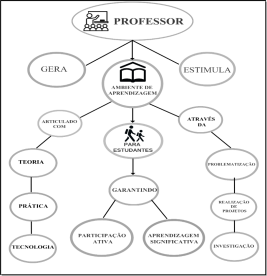
\includegraphics[width=0.5\textwidth]{Fig01.png}
 \caption{O Princípio Educativo.}
 \label{Fig01}
 \source{Do autor, 2020.}
\end{figure}

De acordo com \textcite[p. 8]{rojo_multiletramentos_2012} “se os textos da contemporaneidade mudaram, as competências/capacidades de leitura e produção de textos exigidas para participar de práticas de letramento atuais não podem ser as mesmas”. Assim, podemos afirmar, então, que na contemporaneidade o modelo emergente de ensino/aprendizagem de leitura e escrita passa a ser o modelo básico da educação e que presume a utilização de novos mecanismos de leitura apresentados em diferentes linguagens e incorporados às tecnologias para a realização de uma aprendizagem eficaz e eficiente.  

\subsection{Interfaces entre a convergência tecnológica e digital, a educação remota e os alunos com TDAH que frequentam os anos finais do Ensino Fundamental}\label{sec-interfaces}
A partir da década de 90 a utilização da Internet foi difundida em escala global a partir de navegadores como Firefox, Internet Explorer, Google Chrome, Safari e Opera que, atualmente, são os mais utilizados. Estes navegadores são uma espécie de ponte entre o usuário e o conteúdo virtual que alcançou pessoas e lugares numa velocidade superior a qualquer outro meio comunicativo. Segundo Paletta e Mucheroni (2014), a primeira geração da Internet chamada de Web 1.0 implantou a popularização das redes sociais como Facebook, Twiter, LinkedIn e Instagram. A Web 2.0, segunda geração, integrou as redes sociais às mídias digitais e às mídias sociais centradas em navegadores, sites de colaboração do internauta, como Wikipedia, YouTube e em sites de relacionamento social. A Web 3.0, termo referente à terceira geração da Internet cunhado por \textcite{markoff_entrepreneurs_2006}, também reuniu todas as redes e mídias digitais e sociais organizando e estruturando informações como títulos, identificações, propriedades e quaisquer outros dados produzidos e acessados através da Internet de maneira cada vez mais rápida e eficiente. Atualmente, é na WEB 3.0, chamada de “WEB Semântica”\footnote{Web Semântica é um movimento colaborativo para organizar a informação de maneira legível para computadores e máquinas através de padrões de formatação de dados como o RDF (Resource Description Framework). \url{https://www.organicadigital.com/blog/o-que-e-web-semantica/}.} e de “Internet das Coisas”\footnote{Em outras palavras, a internet das coisas nada mais é que uma rede de objetos físicos (veículos, prédios e outros dotados de tecnologia embarcada, sensores e conexão com a rede) capaz de reunir e de transmitir dados. \url{https://pt.wikipedia.org/wiki/Internet_das_coisas}.}, que a nova geração de crianças, jovens e adultos utiliza um único dispositivo conectado à Internet para acessar repositórios de informações disponíveis em diferentes fontes, conversar trivialmente, conhecer pessoas, comunicar-se com amigos distantes e estabelecer remotamente a aprendizagem por meio de trocas colaborativas.  Essa geração conectada leva o nome de “Nativos digitais”\footnote{Um nativo digital é aquele que nasceu e cresceu com as tecnologias digitais presentes em sua vivência. \url{https://pt.wikipedia.org/wiki/Nativodigital}.}, e podemos afirmar que a convergência tecnológica e digital ocorreu através de práticas de leitura e escrita mediadas por écrans, telas e interfaces oferecidas pela WEB 3.0. 

\textcite[p. 28]{goulart__2011} declara que: 

\begin{quote}
    Apesar do conhecimento da escrita em si permanecer o mesmo como uma forma de linguagem, as novas condições de produção da informação digital determinam outras formas de organização do discurso, novos gêneros, novos modos de ler e de escrever.
\end{quote}

Em suma, se antes a indagação era como se comunicar e ter acesso às informações, hoje elas estão por toda parte sendo transmitidas pelas redes sociais, pelas mídias digitais e pelas mídias sociais e, em tempos de novos tipos de letramento, nos deparamos com um novo formato linguístico de leitura e escrita amparados pelas TDICs que buscam meios de informar. Segundo \textcite[p. 32]{furtado_os_2000}, “Trata-se de um deslocamento na experiência fundamental de ler e de escrever”, e é neste novo cenário que surge, também, a discussão sobre os multiletramentos e os novos letramentos.          

De acordo com \textcite[p. 65]{coscarelli_multiletramentos_2019}:

\begin{quote}
    Pensar a educação sob essa perspectiva nos leva a considerar, inevitavelmente, a noção de multiletramentos em suas concepções mais frequentes, ou seja, o trabalho com vários canais de comunicação e mídias, o que leva ao trabalho com múltiplas linguagens, assim como o trabalho e o respeito à diversidade linguística e cultural que integram esses meios.
\end{quote}

Como dito no item 2, podemos afirmar que ler em tempos de conectividade pressupõe a utilização de novos mecanismos de leitura apresentados em diferentes linguagens e incorporados às tecnologias. Daí a importância do letramento digital. 

De acordo com \textcite{rojo_letramentos_2019}, atualmente para se adequar às novas configurações da Web professores e alunos precisam adquirir quatro tipos de letramento digital, são eles:
 
\begin{enumerate}[label={\alph*}]
    \item o letramento relacionado ao uso da linguagem para comunicação, que inclui aparelhos celulares, tabletes, \textit{e-books}, entre outros; 
    \item o letramento para utilizar adequadamente a ferramenta de “busca e filtragem de informação” oferecida por várias páginas HTML; 
    \item o letramento que faz com que os indivíduos usem os famosos “emojis” ou “memes” como linguagem semiótica para serem compartilhadas em redes sociais;
    \item e o letramento que inclui o (re-)desenho ou remix, como editores de imagens, inserção de voz ou legendas em filmes etc. 
\end{enumerate}

\textcite{rojo_pedagogia_2016} ainda declara que todos estes tipos de letramento são necessários, pois atualmente nossos hábitos de leitura sofreram uma mudança importante, se observarmos que a leitura de livros tem sido gradativamente substituída pela leitura realizada em suportes tecnológicos como aparelhos celulares, \textit{tablets}, \textit{ebooks} etc., com o auxílio de aplicativos digitais e em meios hipermidiáticos, multimodais e multissemióticos.

De acordo com \textcite{menezes_tecnologias_2019}\footnote{Em seu artigo “Tecnologias digitais no ensino de línguas: passado, presente e futuro”, \textcite{menezes_tecnologias_2019} amplia a lista de contingências de uso digital e tecnológico voltadas para a educação apresentada por \cite[p. 197]{gee_anti-education_2013}.}:

\begin{quote}
    [...] em nosso contexto, há professores e alunos utilizando, para fins educacionais:
    \begin{itemize}
\item Messenger e Whatsapp e, cada vez menos, o e-mail para interações acadêmicas e educacionais;
\item Whatsapp para trabalhos em grupo;
\item Skype para interações por vídeo e voz em tempo real para atividades acadêmicas, como, por exemplo, defesas de trabalhos finais de curso;
\item Dropbox, icloud e outros espaços virtuais para armazenamento de dados;
\item Corpora públicos para consulta e estudos sobre diversas línguas, como, por exemplo, o Corpus of Contemporary American English (COCA), disponível em: \url{http://corpus.byu.edu/coca/};
\item Dicionários eletrônicos;
\item Aplicativos para aprendizagem de línguas;
\item Redes sociais para atividades pedagógicas, como, por exemplo, o Facebook;
\item Formulários eletrônicos, como, por exemplo, Survey Monkey, para criação de questionários e coleta de informações;
\item Google docs e ferramentas Wiki\footnote{WIKI, palavra haitiana, wiki wiki, que significa “Rápido” em PB} para escrita colaborativa;
\item Google Drive para compartilhamento de material;
\item Ferramentas de apresentação como Power Point e Prezi;
\item Jogos na web;
\item Rádio na web;
\item Ambientes virtuais de aprendizagem como o Moodle;
\item Youtube e outros repositórios de vídeos para publicação de aulas, tutoriais e atividades realizadas pelos estudantes;
\item Publicação de objetos de aprendizagem de acesso aberto (ver o projeto ELO do Prof. Vilson Leffa, disponível em \url{http://www.elo.pro.br/cloud/});
\item Software para aprendizagem de línguas (ver levantamento de \textcite{borges_are_2014}). \cite[p. 18]{menezes_tecnologias_2019}.
    \end{itemize}
\end{quote}

E, para \textcite[p. 151]{soares_praticas_2002}, o letramento digital é “[...] um certo estado ou condição que adquirem os que se apropriam da nova tecnologia digital e exercem práticas de leitura e de escrita na tela [...]”. \textcite{soares_praticas_2002} ainda afirma que o letramento digital é uma nova concepção que compreende as práticas de leitura e escrita na era da Web Semântica e que corresponde ao processo de desenvolvimento de competências e habilidades para comunicação e localização de informações no ambiente virtual. 

Vimos, portanto, que a informação foi tecnologicamente democratizada, porém, sabemos que, no Brasil, em termos educacionais, existe uma ilusória unanimidade de alegações democráticas, pois as condições de acesso por questões socioeconômicas refletem em desigualdades relacionadas, principalmente, à aquisição de conhecimento e de habilidades. Neste sentido, o novo desafio frente ao contexto emergente de aprendizagem será, então, saber como “minimizar a exclusão de muitos sujeitos já excluídos em muitas outras situações”, \textcite[p. 27]{coscarelli_letramento_2007}, e orientar, remotamente, alunos com TDAH que frequentam os anos finais do Ensino Fundamental a internalizar toda a informação oferecida pela proliferação de mídias digitais e sociais para transformá-la em conhecimento. 

\subsubsection{Mas, afinal, o que vem a ser TDAH?}\label{sec-TDAH}
O Transtorno do deficit de atenção com hiperatividade é um distúrbio que prevalece na infância e na adolescência que tem como características principais a hiperatividade, a presença contínua de desatenção e a impulsividade. O indivíduo com TDAH tem dificuldade em manter-se concentrado. Pode-se dizer que esta é a característica principal. Para alguns pesquisadores este problema tem sua origem em uma condição orgânica relacionada a uma estrutura cerebral chamada lobo pré-frontal. Segundo \textcite[p. 64]{andrade_transtorno_2018}:

\begin{quote}
    [...] é um distúrbio prevalente na infância e adolescência, cujo diagnóstico requer anamnese detalhada e exame físico completo, uso de escalas comportamentais e a consideração plena do diagnóstico diferencial. O tratamento multidisciplinar e multifatorial do transtorno visa à modificação comportamental e reorganização individual, objetivando o desempenho funcional satisfatório em todos os ambientes sociais.
\end{quote}

O TDAH foi considerado por \textcite[p. 231]{carvalho_disturbios_2007} como um “distúrbio de aprendizagem” caracterizada por: 

\begin{quote}
    uma perturbação no ato de aprender, isto é, uma modificação dos padrões de aquisição, assimilação e transformação, sejam por vias internas ou externas do indivíduo. Acrescentando, distúrbios de aprendizagem como sendo uma disfunção do Sistema Nervoso Central relacionada a uma 'falha' no processo de aquisição ou do desenvolvimento, tendo, portanto, caráter funcional, sendo assim, um distúrbio não caracteriza uma ausência, mas sim uma perturbação dentro de um processo; assim, qualquer distúrbio implica em uma perturbação na 'aquisição, utilização e armazenamento de informações, ou na habilidade para soluções de problemas'. Portanto, os distúrbios de aprendizagem seriam uma perturbação no ato de aprender, isto é, uma modificação dos padrões de aquisição, assimilação e transformação, sejam por vias internas ou externas ao indivíduo.
\end{quote}

Porém, atualmente o termo “Distúrbio de Aprendizagem” foi substituído pelo termo Transtorno Funcional Específico (TFE) por recomendação da Política Nacional de Educação Especial (PNEE) que enfatiza a visão pedagógica em contraposição a visão médica. De acordo com a Associação Brasileira do Déficit de Atenção (ABDA), a primeira descrição do que hoje é intitulado de TDAH foi em 1902. Este TFE tem características neurobiológicas podendo ser hereditárias. O TDAH é reconhecido oficialmente por vários países e pela Organização Mundial da Saúde (OMS), e em alguns países os indivíduos com TDAH recebem tratamento diferenciado na escola. A quinta edição do DSM-5 (Diagnostic and Statistical Manual of Mental Disorders) apresenta três tipos de TDAH, são eles: 

\begin{enumerate}
    \item Desatenção predominante - é caracterizado como inquieto porque dificilmente fica parado por muito tempo em um mesmo lugar. Presta pouca atenção em detalhes e comete erros. Muitas vezes distrai-se por qualquer coisa (um barulho, um pensamento, entre outros estímulos). Tem dificuldade de concentração em aulas, palestras, leitura. Pode apresentar problemas de memória em curto prazo (esquece nomes, prazos, datas, perde ou esquece objetos e, até mesmo, o que ia dizer) e quando é chamado, às vezes, parece não ouvir;
    \item Hiperatividade/impulsividade predominante – o indivíduo do tipo hiperativo-impulsivo apresenta inquietação, tenta realizar várias coisas ao mesmo tempo (não suporta situações tediosas), tende a interromper a fala de outras pessoas, por ser impaciente responde aos questionamentos antes de o emissor concluir as perguntas. Ao falar é prolixo e perde a objetividade, mas não se dá conta disso;
    \item Combinado - Apresenta as características combinadas Tipo Hiperativo-Impulsivo e Tipo Desatento predominante.
\end{enumerate}

Segundo \textcite{goncalves_inclusao_2019}, um dos critérios para que uma criança seja diagnosticada com TDAH é que os sintomas apresentem-se em pelo menos dois ambientes: em casa e na escola. E, segundo \apud{pain_diagnostico_1985}[p. 111]{costa_estrategias_2015}: 

\begin{quote}
    As dificuldades de aprendizagem geralmente são percebidas com o ingresso da criança no ensino formal e caracteriza-se por manifestações significativas na aquisição e utilização da compreensão falada, auditiva, da leitura, da escrita e do raciocínio lógico. Sua causa pode estar associada a fatores intrínsecos e extrínsecos ao indivíduo e traz consequências em outros aspectos como na autorregulação do comportamento, percepção social, bem como na interação social.
\end{quote}

\textcite[p. 48]{goncalves_inclusao_2019} afirma também que “A família, como responsável pela educação das crianças, deve participar ativamente do seu processo de desenvolvimento.”. Em sua pesquisa, \textcite{goncalves_inclusao_2019} observou que apenas cinquenta por cento das famílias acompanham a vida escolar de filhos com TDAH e considerou esse dado alarmante, pois acredita que a família precisa se conscientizar de que existem maneiras adequadas para lidar com crianças que apresentam esse tipo de TFE.  

De acordo com \textcite{antunes_glossario_2001}, em seu Glossário para educadores, a falta de conhecimento de educadores e/ou de pais sobre o TDAH prejudicam substancialmente o desenvolvimento das crianças com este tipo de TFE. Para \textcite[p. 140]{antunes_glossario_2001}:

\begin{quote}
    Muitas crianças que pais e professores normalmente rotulam de “hiperativas” são apenas mais ativas que seus pais e professores foram ou desejariam que fossem. A hiperatividade somente se manifesta quando existem comprometimentos na manutenção da atenção para diferentes atividades.  A criança, por exemplo, que não presta atenção à aula, mas presta muita atenção ao jogo, não revela distúrbio de atenção, típico da hiperatividade. A hiperatividade pode ser tratada com drogas relacionadas ao grupo das anfetaminas, somente ministradas por especialistas após a óbvia constatação dessa condição. Em muitos casos a hiperatividade permanece até o final da adolescência.
\end{quote}

No atual contexto educacional, no qual se faz necessário o Ensino Remoto Emergencial devido ao distanciamento social orientado pela OMS em função do vírus pandêmico SARS CoV-2, a tecnologia tem contribuído para a reflexão sobre os possíveis usos sociais e práticas inclusivas da leitura e da escrita em diferentes modalidades educacionais, pois este cenário emergente de ensino/aprendizagem exige que se pense também numa ação que seja efetiva e transformadora e que estimule os indivíduos com TDAH a criarem familiaridade com a leitura e com a escrita, ainda que remotamente, fazendo com que este indivíduo, além de ser inserido em ambientes educativos com a presença de artefatos tecnológicos, seja capaz de compreender e construir a sua própria realidade. 

A partir destas considerações, devemos passar a enxergar o universo virtual como uma oportunidade importante para a formação do leitor digital, não como uma ameaça, pois esse ciberespaço traz consigo desafios incontestáveis de aprendizagem que vieram para ficar, além de colocar à disposição um mundo de informações em contexto de interatividade. Porém, neste contexto pandêmico, que exigiu a aplicação da modalidade de Ensino Remoto Emergencial, percebemos que a maioria das ferramentas digitais e apps não foi desenvolvida propriamente para o uso de alunos com TDAH que frequentam os anos finais do EF. 

\subsubsection{Integração e inclusão em tempos de conectividade}\label{sec-integracao}
Para que uma ação educacional remota voltada para alunos com TDAH seja efetiva e transformadora é necessário diferenciar “integração” de “inclusão”. 

De acordo com \textcite[p. 2]{borgesdalberio_inclusao_2012}:

\begin{quote}
    [...] integração escolar, cuja metáfora é o sistema de cascata, é uma forma condicional de inserção em que vai depender do aluno, ou seja, do nível de sua capacidade de adaptação às opções do sistema escolar, a sua integração, seja em uma sala regular, uma classe especial, ou mesmo em instituições especializadas. Trata-se de uma alternativa em que tudo se mantém, nada se questiona do esquema em vigor”.
\end{quote}

Neste sentido, a integração está relacionada com a participação ampliada dos indivíduos na escola. Significa permitir que alunos normalmente excluídos (que possuem NEE entre outros) participem das turmas consideradas regulares, isso requer que o aluno se adapte ao ritmo da escola. 

Sobre inclusão escolar, \textcite{stainback_inclusao_1999} afirmam que:

\begin{quote}
    A educação inclusiva pode ser definida como a prática da inclusão de todos – independentemente de seu talento, deficiência, origem socioeconômica ou cultural – em escolas e salas de aula provedoras, onde as necessidades desses alunos sejam satisfeitas \apud[p. 21]{stainback_inclusao_1999}[p. 87]{silva_neto_educacao_2018}.
\end{quote}

Assim, a integração privilegia o aluno portador de NEE, partilhando com ele a responsabilidade da inserção, enquanto a inclusão tenta avançar, exigindo, também, da sociedade em geral, condições para essa integração. 

Trabalhar com as necessidades específicas de alunos que possuem NEE com o objetivo de promover etapas para que esse aluno possa acompanhar e ter acesso a todas as atividades desenvolvidas na sala regular é um direito assegurado pelo MEC/SEESP através das Diretrizes da Política Nacional de Educação Especial na Perspectiva da Educação Inclusiva \cite{brasil_politica_2008}, ao determinar que:

\begin{quote}
    A educação especial é uma modalidade de ensino que perpassa todos os níveis, etapas e modalidades, realiza o atendimento educacional especializado, disponibiliza os recursos e serviços e orienta quanto a sua utilização no processo de ensino e aprendizagem nas turmas comuns do ensino regular. O atendimento educacional especializado tem como função identificar, elaborar e organizar recursos pedagógicos e de acessibilidade que eliminem as barreiras para a plena participação dos alunos, considerando suas necessidades específicas. As atividades desenvolvidas no atendimento educacional especializado diferenciam-se daquelas realizadas na sala de aula comum, não sendo substitutivas à escolarização. Esse atendimento complementa e/ou suplementa a formação dos alunos com vistas à autonomia e independência na escola e fora dela. Dentre as atividades de atendimento educacional especializado são disponibilizados programas de enriquecimento curricular, o ensino de linguagens e códigos específicos de comunicação e sinalização e tecnologia assistiva.
    
    Ao longo de todo o processo de escolarização esse atendimento deve estar articulado com a proposta pedagógica do ensino comum. O atendimento educacional especializado é acompanhado por meio de instrumentos que possibilitem monitoramento e avaliação da oferta realizada nas escolas da rede pública e nos centros de atendimento educacional especializados públicos ou conveniados. \cite[p. 9]{brasil_politica_2008}.
\end{quote}

Na \cref{Fig02} podemos observar que o próprio PPP (Projeto Político Pedagógico), que é alicerçado em um trabalho pedagógico amparado pela Lei 9394/96, Art. 12, 13, 14 e incisos, pressupõe uma concepção de mundo, homem, sociedade e escola e exige a efetiva participação dos alunos, dos pais, dos professores, da comunidade e do governo municipal, estadual e federal. 

\begin{figure}[htbp]
 \centering
 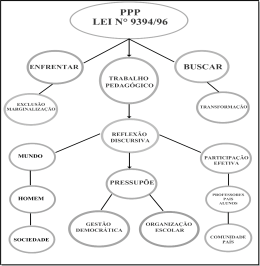
\includegraphics[width=0.5\textwidth]{Fig02.png}
 \caption{PPP (Projeto Político Pedagógico) – Princípios básicos.}
 \label{Fig02}
 \source{Do autor, 2020.}
\end{figure}

No entanto, o Gestrado (Grupo de Estudos sobre Política Educacional e Trabalho Docente/UFMG) em parceria com o CNTE, ao investigar os efeitos das medidas de distanciamento social em função da Covid-19 sobre o trabalho docente na Educação Básica, observou que 90\% dos professores da Educação Básica não têm experiência com aulas remotas e que a maioria dos profissionais da educação não receberam qualquer formação para o desenvolvimento de atividades remotas com artefatos tecnológicos. Consequentemente, podemos afirmar que estes professores também não estão preparados para integrar e incluir os alunos que possuem NEE, como o TDAH, à nova realidade tecnológica de educação. 

A \cref{Fig03} mostra o índice de formação específica em aulas remotas para grande parte dos docentes da Educação Básica. 

\begin{figure}[htbp]
 \centering
 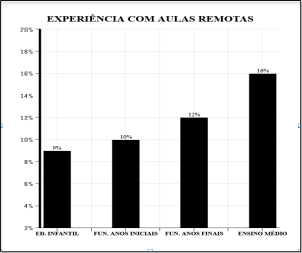
\includegraphics[width=0.5\textwidth]{Fig03.png}
 \caption{Professores e aulas remotas.}
 \label{Fig03}
 \source{Adaptado de \cite{oliveira_trabalho_2020}}.
\end{figure}

Em outro levantamento realizado pelo Portal G1\footnote{\url{https://g1.globo.com/educacao/noticia/2020/07/06/60percent-dos-estados-monitoram-acesso-ao-ensinoremoto-    resultados-mostram-apagao-do-ensino-publico-na-pandemia.ghtml}.} em 06 de julho de 2020 junto às secretarias estaduais de educação mostra que, após os primeiros 100 dias de suspensão das aulas presenciais pelo país devido à pandemia causada pelo novo coronavírus SARS COVID-2, apenas 15 dos 25 estados que implantaram atividades à distância monitoraram a adesão dos estudantes ao ensino remoto. Segundo o Portal G1, as aulas \textit{on-line} não são acompanhadas por todos os alunos, e declara ainda que:

\begin{quote}
    Isso significa que, apesar dos esforços das redes, parte dos estudantes pode não ter acesso à educação durante a pandemia. As razões são várias – e incluem falta de estrutura em casa, de computadores ou de conexão. A alternativa para os alunos é recorrer às atividades impressas ou à transmissão por outras mídias, como TV aberta ou via rádio. Nesses casos, também é difícil mensurar quantos estudantes estão efetivamente assistindo ao conteúdo.
\end{quote}

É neste momento que o PPP deve sugerir uma organização escolar que se proponha a incentivar todos os atores envolvidos na educação a realizarem uma discussão reflexiva sobre todos os conceitos buscando uma transformação social a partir de uma gestão democrática que evite e enfrente a exclusão e a marginalização das nossas crianças, dos nossos jovens e dos nossos adolescentes.

De acordo com \textcite[p. 21]{oliveira_trabalho_2020}:

\begin{quote}
    o compromisso desses professores(as) com seus estudantes tem orientado a busca de meios para tornar a oferta educativa possível. Essa experiência pode significar um importante crescimento e amadurecimento profissional, mas ela também é geradora de tensões e angústias para os docentes", aponta o documento.
\end{quote}

A partir dos dados apontados, surge, então, a necessidade de encontrar profissionais especializados que sejam capazes de utilizar as TDICs, desde a Educação Infantil, com o objetivo de integrar e incluir os indivíduos que possuem NEE à nova modalidade de Ensino Remoto Emergencial. Sob tais circunstâncias, é imprescindível que este profissional conheça e domine as inúmeras possibilidades que a aprendizagem emergencial e o mundo conectado podem oferecer e que elabore situações de aprendizagem que levem em consideração o contato sistemático deste aluno com o universo virtual para que ocorra a aquisição eficaz e eficiente do letramento digital. 

\section{Método e aplicação}\label{sec-metodo}
Para realização deste artigo, foi realizada uma pesquisa bibliográfica de abordagem qualitativa sobre alunos com TDAH matriculados nos anos finais do Ensino Fundamental e sobre pesquisas que abordam a leitura e alfabetização, os Transtornos Funcionais Específicos (TFEs), a educação mediada pela tecnologia, a educação especial e a educação inclusiva, pautando-nos em estudos de pesquisadores como \textcite{alexander_2004, antunes_glossario_2001, borgesdalberio_inclusao_2012, coscarelliribeiro_2005, menezes_tecnologias_2019, silva_neto_educacao_2018, rojo_multiletramentos_2012, rojo_generos_2013, andrade_transtorno_2018, goncalves_inclusao_2019, lopes_inclusao_2011, coscarelliribeiro_2005, rohde_transtorno_1999, amorim_TDAH}, entre outros. 

Como vimos, a tríade comportamental de desatenção, hiperatividade/impulsividade ou a combinação das duas últimas geralmente é percebida após o ingresso do indivíduo com TDAH no ambiente escolar, uma vez que, é no período escolar que comportamentos característicos deste tipo de transtorno funcional específico ficam em evidência e resultam em dificuldades de aprendizagem, \cite{pain_diagnostico_1985}. Seguindo as orientações dos pesquisadores de TFEs, para suprir as dificuldades apresentadas pelos alunos com TDAH que frequentam os anos finais do EF temos que considerar as seguintes questões:

\begin{enumerate}[label={\alph*}]
    \item Tarefas que demandam muito tempo para realização devem ser dispensadas, pois, de maneira geral, estes alunos costumam se distrair com essas tarefas, exigindo um tempo maior para conseguir finalizá-las.
    \item Alunos com TDAH possuem uma necessidade maior de “gastar energia”, de forma que o tempo de aula no qual devem ficar sentados, torna-se um desafio, por isso devem ser evitadas aula com conteúdos longos.  É comum que o estudante que se enquadra neste tipo de TFE procure sair da sala com mais frequência (pedidos constantes para beber água ou utilizar o banheiro) ou que levante para pegar algum material emprestado com o colega que está em outra parte da sala.
    \item Alunos com TDAH necessitam de maiores estímulos para construir conhecimento e, além disso, por apresentarem inteligência média ou acima da média e terem dificuldades para seguir orientações, \textcite{rohde_transtorno_1999}, os alunos com TDAH dos anos finais do EF devem preferencialmente realizar uma atividade de cada vez e concluir uma etapa para iniciar outra.
    \item Nos anos finais do EF os alunos com TDAH ficam mais motivados e atentos quando são realizadas atividades lúdicas, que movimentam o corpo ou quando as orientações são dadas em etapas.
    \item É comum que os professores do EF disponibilizem em suas aulas uma grande quantidade de informações, porém, para os alunos com TDAH o fluxo das atividades deve ser variado, pois a monotonia da mesma atividade por um longo período faz com que este aluno fique estressado e cada vez mais desinteressado 
\end{enumerate}

\subsection{Sites que podem ser utilizados por alunos com TDAH que frequentam os anos finais do Ensino Fundamental II}\label{sec-sites}

\subsubsection{YouTube}\label{sec-youtube}
O YouTube\footnote{\url{https://www.youtube.com/}} é uma plataforma de compartilhamento de áudios e vídeos em rede social e sua principal função é permitir que os usuários façam downloads,1 assistam e compartilhem qualquer tipo de vídeo que esteja em formato digital. Vale destacar os chamados “canais”, um novo fenômeno que ganhou ampla proporção entre os jovens que utilizam estes meios para o compartilhamento de informações através do YouTube. 

A contação de histórias via YouTube é uma ferramenta que pode ser utilizada para ganhar a atenção de alunos com TDAH dos anos finais do Ensino Fundamental. Você já assistiu a alguma contação de história pelo YouTube? Os internautas usam a internet para falar sobre as histórias dos livros que estão lendo ou que gostariam de ler. Eles fazem a contação de histórias de um modo bastante descontraído e descompromissado. Todos os dias, surgem novos segmentos com diferentes conteúdos abordados. O tradicional “joinha” no final do vídeo traduz a satisfação ou não satisfação do material compartilhado, e já faz parte desta realidade das linguagens mediadas pelo cenário do ciberespaço. 

Apesar das particularidades desta rede social, o uso de vídeos \textit{on-line} para contação de histórias é uma maneira de apresentar este espaço como uma possibilidade para ampliar o universo literário de alunos com TDAH inseridos nos anos finais do Ensino Fundamental, além de se caracterizar como fonte para conhecer novas histórias e divulgar novos autores que, muitas vezes, estão fora do universo das editoras. Como exemplo de vídeos que podem ser trabalhados remotamente ou dentro de sala com alunos que possuem ou não necessidades especiais de aprendizagem temos: 

\begin{itemize}
    \item Contos Infantis
    \subitem Contos de Fadas com a Gigi\footnote{\url{http://contosdefadascomagigi.com}};
    \subitem A Raposa e a Cegonha | Fabula | Desenho animado infantil com os Amiguinhos\footnote{\url{https://youtu.be/gNnb0pMEc6s}};
    \subitem Contos Juvenis
    \subitem Contação de história - O Vestido Azul\footnote{\url{https://www.youtube.com/watch?v=D368BPqCpLk}};
    \subitem Contação de História - Até as Princesas Soltam Pum - História Infantil Narrada\footnote{\url{https://www.youtube.com/watch?v=h8qyceMMltk&t=53s}}.
\end{itemize}

\subsubsection{Trello}\label{sec-trello}

O Trello\footnote{\url{https://www.trello.com.br}} é uma ferramenta de gerenciamento de projetos que pode ser utilizada como apoio pedagógico para o professor que leciona para alunos com TDAH nos anos finais do EF. Essa ferramenta pode ser acessada através dos principais navegadores como Google Chrome, Mozilla Firefox, Safari ou Internet Explorer através dos apps Google Play e iTunes e não precisa ser instalada nos suportes digitais. Desenvolvida para criar quadros, tarefas e atividades para as turmas, essa ferramenta permite um trabalho em equipe e pode ser utilizada para acompanhar o desenvolvimento dos alunos. Para alunos que com TDAH matriculados nos anos finais do Ensino Fundamental, essa ferramenta pode estimular a organização pessoal, uma vez que, permite a visualização de todas as tarefas pendentes definindo a situação de cada uma (se estão em andamento, concluídas ou para iniciar). 

\subsubsection{Blogs}\label{sec-blogs}
Escolhemos o Blog como ferramenta de ensino/aprendizagem voltada para alunos com TDAH que estejam matriculados nos anos finais do Ensino Fundamental porque ela permite, não só a publicação de conteúdo digital, mas também apresenta alguns mecanismos para o desenvolvimento da escrita, da leitura e da criatividade. Além disso, esses alunos podem interagir com todos os colegas de sala de aula ao serem incentivados a criar os blogs.

De acordo com \textcite[p. 8]{girafa_reinvencao_2012}:

\begin{quote}
Utilizar blogs como uma ferramenta para criação de conteúdo digital não apenas pelo professor, mas também pelos seus alunos, possibilitará ao docente compreender o nível de aprendizagem e motivará o aluno a aprender coisas novas além de mostrar àqueles que estão fora da escola a autoria de seus projetos.  
\end{quote}

A produção de blogs é bem simples, mas, assim como as ferramentas e apps citados anteriormente, exige uma certa autonomia por parte do alunado. A estrutura dos Blogs permite atualização diária dos dados. É possível publicar artigos de assuntos específicos ou variados, imagens, músicas, entre outros que o administrador preferir compartilhar. Sua estrutura permite também a atualização rápida a partir de acréscimos dos chamados artigos ou \textit{posts}, possibilitando que o leitor/escritor expresse seus interesses e proporcione um espaço de trocas informacionais. Essa prática é uma maneira de ampliar o sentido de leitura e da escrita, ao apresentar um novo arranjo textual e incentivar a interpretação de textos no formato virtual. A atenção dos alunos dos anos finais do Ensino Fundamental que apresentam TDAH será controlada principalmente se os blogs forem montados com assuntos que mais lhe interessam. Basta que o professor tenha um conhecimento prévio sobre os hábitos desses alunos. Os Blogs, então, podem surgir no processo de aprendizagem educacional tanto relacionado à prática da pesquisa e aquisição informacional como ferramenta para o desenvolvimento da leitura, da escrita e da criatividade. Em alguns blogs as conversas podem se debruçar na “tessitura do texto" que têm o objetivo de fazer com que o aluno perceba que a atividade de produção textual sempre esteve relacionada à de leitura. 

\subsubsection{AVA}\label{sec-ava}
São inúmeras as possibilidades que os alunos possuem para fazer uso das funções de seus suportes digitais em sala de aula. Através destes aparelhos, os alunos podem acessar conteúdo online e trocar informações em tempo real. Pode-se, também, acessar Ambientes Virtuais de Aprendizagem, os (AVA’s). Um AVA é um site na web que permite realizar, em um único espaço, ações próprias do processo de ensino e aprendizagem. Alunos do EF com TDAH podem utilizar essa ferramenta para construir conhecimento. Um AVA é um ambiente que tem a capacidade de oferecer condições de aprendizagem para todos aqueles que fazem parte de uma sala de aula. Esses ambientes possuem inúmeras ferramentas, como roteiros, fóruns, chats, compartilhamento de documentos e sistemas de avaliação que permitem o acompanhamento das atividades didáticas de maneira semelhante a outros espaços educacionais. Atualmente existem diversas opções de AVA. Alguns são gratuitos e outros pagos. Podem ser de software livre ou locador. Cada um dispõe de facilidades diferentes. O melhor AVA será escolhido de acordo com as necessidades de cada sistema de ensino. São muitos os AVA’s. Listaremos alguns exemplos mais utilizados. 

\begin{enumerate}[label={\alph*}]
    \item Moodle - ambiente modular de aprendizagem dinâmica orientada a objetos baseada num software livre;
    \item MOOCs – assim como os AVA’s são cursos online abertos desenvolvidos por instituições acadêmicas e acessíveis à qualquer pessoa que tenha acesso à internet. 
    \item Edmodo é uma plataforma educacional que permite compartilhar conteúdos, organizar debates, realizar votações, dispor de uma agenda. 
\end{enumerate}

\subsection{Jogos}\label{sec-jogos}
Segundo \textcite{antunes_glossario_2001}, “A criança, por exemplo, que não presta atenção à aula, mas presta muita atenção ao jogo, não revela distúrbio de atenção, típico da hiperatividade”. E, de acordo com \textcite[p. 64]{lopes_inclusao_2011}: 

\begin{quote}
    O jogo virtual é uma ferramenta criativa, atraente e interativa que auxilia o professor a minimizar os problemas de desatenção e de comportamento social nos alunos com TDAH, potencializando a aprendizagem e, consequentemente, seu desenvolvimento cognitivo.
\end{quote}

A partir de tais considerações, podemos afirmar que jogos virtuais, nas suas diversas formas, são uma outra atividade funcional que pode ser utilizada nos anos finais do EF para o trabalho junto à criança com TDAH. Como exemplo de jogos virtuais voltados para alunos com TDAH matriculados nos anos iniciais e finais do EF, temos:

\subsubsection{Brainy Mouse}\label{sec-brainy}
O Brainy Mouse\footnote{\url{https://playtable.com.br/jogos/brainy-mouse}} é um jogo disponível para suportes tecnológicos e digitais com sistema operacional Android e IOS. É uma ferramenta que pode ser utilizada por crianças em faixa etária de alfabetização. A proposta deste jogo é apresentar uma cozinha de restaurante na qual os jogadores devem completar as receitas realizando a formação de palavras, buscando dicas em sílabas, cores, sons e gráficos. Essa ferramenta é muito atrativa para alunos com TDAH, tanto dos anos iniciais quanto dos anos finais do EF, por apresentar muitos elementos que chamam a atenção e que permitem que eles fiquem concentrados no jogo por um período maior do que ficariam em atividades tradicionais, pois, como vimos, a monotonia da mesma atividade por um longo período faz com que este aluno fique estressado e cada vez mais desinteressado.

\subsubsection{Brain n-Back; Brain test; Cognifit Brain Fitness; Lumosity; Mind Games; Peak e Skillz}\label{sec-brainn}
Estes APPs são jogos capazes de atrair atenção dos alunos por proporcionar desafios que necessitam de atenção aos detalhes da cena representada. Disponíveis para suportes com Android e IOS estes jogos trabalham a memória, a concentração e a capacidade de seguir instruções que é uma questão difícil para os alunos com TDAH que frequentam os anos finais do E. Apesar de não trabalhar diretamente com conteúdo pedagógico, estes jogos podem facilitar e melhorar a vida desses estudantes.

\subsection{Bloqueadores}
Em tempos de \textit{home office}, os pais de alunos em idade escolar precisam acompanhar os estudos de seus filhos e fazer com que distrações durantes aulas remotas não ocorram. Sabemos que alunos com TDAH dos anos finais do EF dispersam constantemente a atenção e isso atrapalha a realização das tarefas e, para sanar este problema, existem várias ferramentas que bloqueiam aplicativos que podem ser utilizados durante pesquisas ou aulas remotas que fazem com que alunos com THAD matriculados nos anos finais do EF consigam utilizar quaisquer ferramentas dos seus suportes, porém sem acessar redes sociais e outros aplicativos durante as atividades. São Eles: Forest; Siempo; Stay on Task; Flipd; AppBlock; Block \& Focus.


\section{Considerações finais}\label{sec-consideracoes}
Ao observar as especificidades e contribuições do letramento digital e da alfabetização inclusiva no processo de ensino e aprendizagem, este estudo revelou que podemos e devemos utilizar os novos suportes multimodais para modificar a relação que os indivíduos que possuem NEE, como o TDAH, têm com a leitura e com a escrita através do Ensino Remoto Emergencial. Além disso, considerando que dispositivos multimodais são utilizados em muitos ambientes escolares para a realização do ensino de escrita e de leitura, observamos também que existe a possibilidade de fazer com que os indivíduos que possuem NEE sejam capazes de se adequar ao Ensino Remoto Emergencial e lidar com os novos usos sociais dos livros seguindo o modelo emergencial de ensino/aprendizagem. Neste sentido, após apresentar algumas possibilidades de trabalhos que utilizam as tecnologias digitais, concluímos que, além de respeitar as diferenças, é dever da escola, do professor, da família e da sociedade criar as condições para que os alunos que possuem NEE interajam espontaneamente em qualquer modalidade educacional, pois quando existe organização e planejamento a sociedade se completa determinando o vínculo entre as pessoas. 

Concluímos também que na atual realidade cibernética, num momento em que o mundo passa por uma mudança de modalidade de ensino devido ao distanciamento social causado pela COVID-19 e, ao mesmo tempo, por uma progressiva convergência de tecnologias digitais, não é mais possível que educadores ignorem a necessária interação de alunos que apresentam NEE com o universo virtual. Este público está conectado, mas precisa ter uma nova postura diante deste tipo de texto. Além disso, as TDICs já estão presentes no dia a dia das escolas, mesmo que não estejam incorporadas ao ensino e à aprendizagem, e cabe a nós educadores considerar o princípio básico da educação contemporânea que pressupõe a utilização de novos mecanismos de leitura apresentados em diferentes linguagens e incorporados às tecnologias para a realização de uma aprendizagem eficaz e eficiente realizada através de meios hipermidiáticos, multimodais e multissemióticos. Isto posto, o uso das TDICs, seja no processo de aprendizagem, seja no aprimoramento das atividades pedagógicas ou na ampliação do material didático, é uma realidade atual que deve contemplar a “estrutura educacional sob os princípios da modernidade”, \textcite{melo_midia_2008}. 

A partir dessas considerações, podemos afirmar que existe a possibilidade de fazer com que os indivíduos que possuem NEE sejam capazes de se adequar ao ensino remoto e lidar com os novos usos sociais dos livros. Além disso, devemos também passar a enxergar o universo virtual como uma oportunidade importante para a formação de leitores digitais, não como uma ameaça, pois esse ciberespaço traz consigo desafios incontestáveis de aprendizagem que vieram para ficar, além de colocar à disposição um mundo de informações em contexto de interatividade. 

A relevância de se estudar o uso das TDICs voltadas para alunos com TDAH que frequentam os anos finais do EF vai muito além da não linearidade do comportamento desse leitor. De acordo com \textcite{tori_educacao_2010}, as novas tecnologias, na verdade, aproximaram as pessoas e possibilitaram ações coletivas antes impensáveis. Estas ações coletivas podem, inclusive, integrar, incluir os alunos com TDAH num espaço que sempre foi seu: o espaço escolar.

\epigraph{Há necessidade de sermos homens e mulheres de nosso tempo que empregam todos os recursos disponíveis para dar o grande salto que nossa educação está a exigir.}{\citefirstlastauthor{freire_educaco_1995}, \textit{\citetitle{freire_educaco_1995}}}

\printbibliography\label{sec-bib}

\end{document}
